\documentclass[a4paper,10pt]{jsarticle}
\usepackage{amsmath,amsfonts}
\usepackage{bm}
\usepackage[dvipdfmx]{graphicx}
\usepackage[dvipdfmx,colorlinks=true,
linkcolor=blue,
filecolor=blue,
urlcolor=blue]{hyperref}
\usepackage{enumerate}
\usepackage{indentfirst}
\graphicspath{{../B/}}


\begin{document}
  \begin{flushright}
    \textbf{\large{Background Assignment}}
  \end{flushright}
  \begin{center}
    \textbf{\large{A. Conceptual Knowledge}}
  \end{center}
  \begin{enumerate}
    \item \textbf{\large{What is a smart contract? How are they deployed? You should be able to describe how a smart contract is deployed and the necessary steps.}}\mbox{}\\
    \newline
    Smart contracts are often compared to vending machines. 
    When you want a drink, you put money in the machine and press a button and the product you have chosen will come out, but if you don't have enough money, the product will not come out.
    In this way,it is smart contract that if certain conditions are met, it automatically formed without the need for an administrator.
    And smart contracts are used in many blockchain protocols, including Ethereum. 
    Smart contracts can be programmed by anyone to be placed on the blockchain and can be combined with other smart contracts. 
    Since they run on a blockchain that cannot be tampered with, contracts and transactions cannot be changed and are secure. 
    Smart contracts can be programmed using specific programming languages. Once programmed, smart contracts can be deployed as follows
    \newline
    \begin{enumerate}[step.1]
      \item program the smart contract (can be written using a specific programming language, e.g. Solidity, Rust)
      \item compile the contract code (convert it to a machine-readable format (Application Binary Interface))
      \item Send the compiled code to the connected network (a Contract account is generated and its address is issued at this time).
    \end{enumerate}\mbox{}\\
    The deployed smart contract can be executed by anyone, who executes the smart contract by issuing a transaction to the Contract account generated during deployment.
    
    The Contract is an immutable computer program and cannot be modified once deployed.
    \newline
    \item \textbf{\large{What is gas? Why is gas optimization such a big focus when building smart contracts?}}\mbox{}\\
    \newline
    It is like fuel used to run smart contracts on ethereum. Why do we need fuel? This is due to the fact that Ethereum is Turing-complete. Turing-complete simply means that it can execute any complex program. In other words, it can run any smart contract! However, this presents a major problem.
    For example, if you had a smart contract (a program that never terminates) that looped infinitely, what would happen if you ran it on ethereum? 
    The participating nodes executing the smart contract could run forever, and the network itself would go down. 
    It has been proven that \textbf{when given an arbitrary program and input, it is impossible to determine if the program will eventually stop (the stoppage problem)}, so it is impossible to reject the program in advance.
    To overcome this difficulty, a lightweight mechanism called "gas" was introduced.
    Every smart contract order has a predetermined cost in units of gas and uses gas (fuel) to run. Naturally, when the gas runs out, the program is forced to terminate, just as a car will stop running when it runs out of fuel. Gas is the fuel needed to run smart contracts on ethereum. 
    \newline
    Consider the command, "Put only one apple in the bag."
    There are two bags, bag A which holds 10 apples (3 ETH for the usage fee) and bag B which holds 2 apples (1 ETH for the usage fee).
    You should not bother to choose bag A, which has a higher usage fee, when the purpose of the bag is to hold one apple. The same can be said for smart contracts. 
    Since gas is paid for by the user who initiates the transaction, smart contracts need to be economically programmed. Since every instruction has a predetermined cost per unit of gas, there are instructions that cost more gas to execute. 
    Basically, a process that costs more gas requires more memory and storage.
    Gas optimization is an unavoidable part of reducing computing resources and economical optimization.
    \newline
    \item \textbf{\large{What is a hash? Why do people use hashing to hide information?}}\mbox{}\\
    \newline
    It is a fixed-length fingerprint that is output for variable-size input.
    Let's look at a concrete example.
    The string "hello world" is hashed using the hash function SHA256.
    \newline
    \newline
    \textrm{b94d27b9934d3e08a52e52d7da7dabfac484efe37a5380ee9088f7ace2efcde9}\mbox{}\\
    \newline
    A fixed-length string of 64 characters was produced.
    Next, we find the hash of the string "hello worle" using the same hash function, just changing "d" to "e".
    \newline
    \newline
    \textrm{0fc30e735a0228a31cbbb969988b4f50e02e737f979f091d7d224b765443f5d4}\mbox{}\\
    \newline
    As before, we get a fixed-length string of 64 characters, but it differs significantly from the hash value we saw earlier. This is a characteristic of hashes.
    A hash has three characteristics.
    \newline
    \begin{enumerate}[1.]
      \item It is almost impossible to identify the original data from the hash value
      \item If the original data is the same, the generated hash value is also the same
      \item If the original data changes by even one bit, the generated hash value will be significantly different.
    \end{enumerate}\mbox{}\\
    There is information that people want to hide in their communications, such as passwords and credit card numbers.
    Let's say you want to use a password, but you don't want to give out your password.
    Suppose the password is "zku".
    If you send zku as it is, the password cannot be hidden. So we use a hash.
    The hash value of "zku" is
    \newline
    \newline
    \textrm{28e4e293086a3925fdb47a089e4ef3eccdeb9032fa63c7a0be430d3a76adb1a8}\mbox{}\\
    \newline
    is. The hash characteristics described above make it almost impossible to identify the "zku" string from this hash value. The fact that the same hash value comes up no matter how many times you type "zku" proves that you know the password. It is also difficult to find an input with the same hash value because the hash value generated will be very different if it changes even by one bit.
    If the hash value in the database and the hash value we sent were identical, we could prove that we knew the password while hiding the information. This is a simple example, but the hash feature can be used to hide a variety of information.
    \newline
    \item \textbf{\large{How would you prove to a colorblind person that two different colored objects are actually of different colors? You could check out Avi Wigderson talk about a similar problem here. }}\mbox{}\\
    \newline
    We prove it by having a dialogue.
    Let the colorblind person be the verifier Alice and the not colorblind person be the prover Bob.
    The following steps are taken
    \newline
    \begin{enumerate}[step.1]
      \item Alice shows two different colored objects to Bob
      \item Where Bob cannot see, Alice swaps or does not swap the two different colored objects
      \item Alice asks Bob if he swapped the position of the objects.
    \end{enumerate}\mbox{}\\
    The key here is step.2: Alice cannot tell the color, but she can identify that the objects have been swapped. This means that only the person who can see the color can always guess whether the objects were swapped, since Bob does not see the moment of the swap.
    The probability of getting it right in one attempt is 1/2.
    Perhaps Bob is colorblind, but he lied and got it right by accident. But what if we repeat this procedure 20 times? The probability of always guessing everything is $\frac{1}{2^{20}}$, which is very low for the probability of guessing the correct answer by chance. 
    20 times in a row you could guess whether or not the two objects were switched, which proves to Alice, who is colorblind, that the two different colored objects are in fact different colors. The important point here is that we are not conveying color information about the objects. 
    We could prove to a colorblind person that two different colored objects are in fact different colors without giving him any information.
     
  \end{enumerate}
  \newpage
  \begin{center}
    \textbf{\large{B. You sure you are solid with Solidity?}}
  \end{center}
  \begin{enumerate}
    \item \textbf{\large{HelloWorld: Program a super simple “Hello World” smart contract: write a storeNumber function to store an unsigned integer and then a retrieveNumber function to retrieve it}}\mbox{}\\
    HelloWorld.sol
    \newline
    Code: \href{https://github.com/Nishino0719/Zero-Knowledge-University/blob/main/BackgroundAssignment/B/HelloWorld.sol}{Code url}\mbox{}\\
    Commit: \href{https://github.com/Nishino0719/Zero-Knowledge-University/commit/f55562e393d832ccb38954473f5d72c46b3ef8be}{Commit code url}\mbox{}\\
    Pull Request:\href{https://github.com/Nishino0719/Zero-Knowledge-University/pull/1/files}{https://github.com/Nishino0719/Zero-Knowledge-University/pull/1/files}
    \begin{figure}[h]
        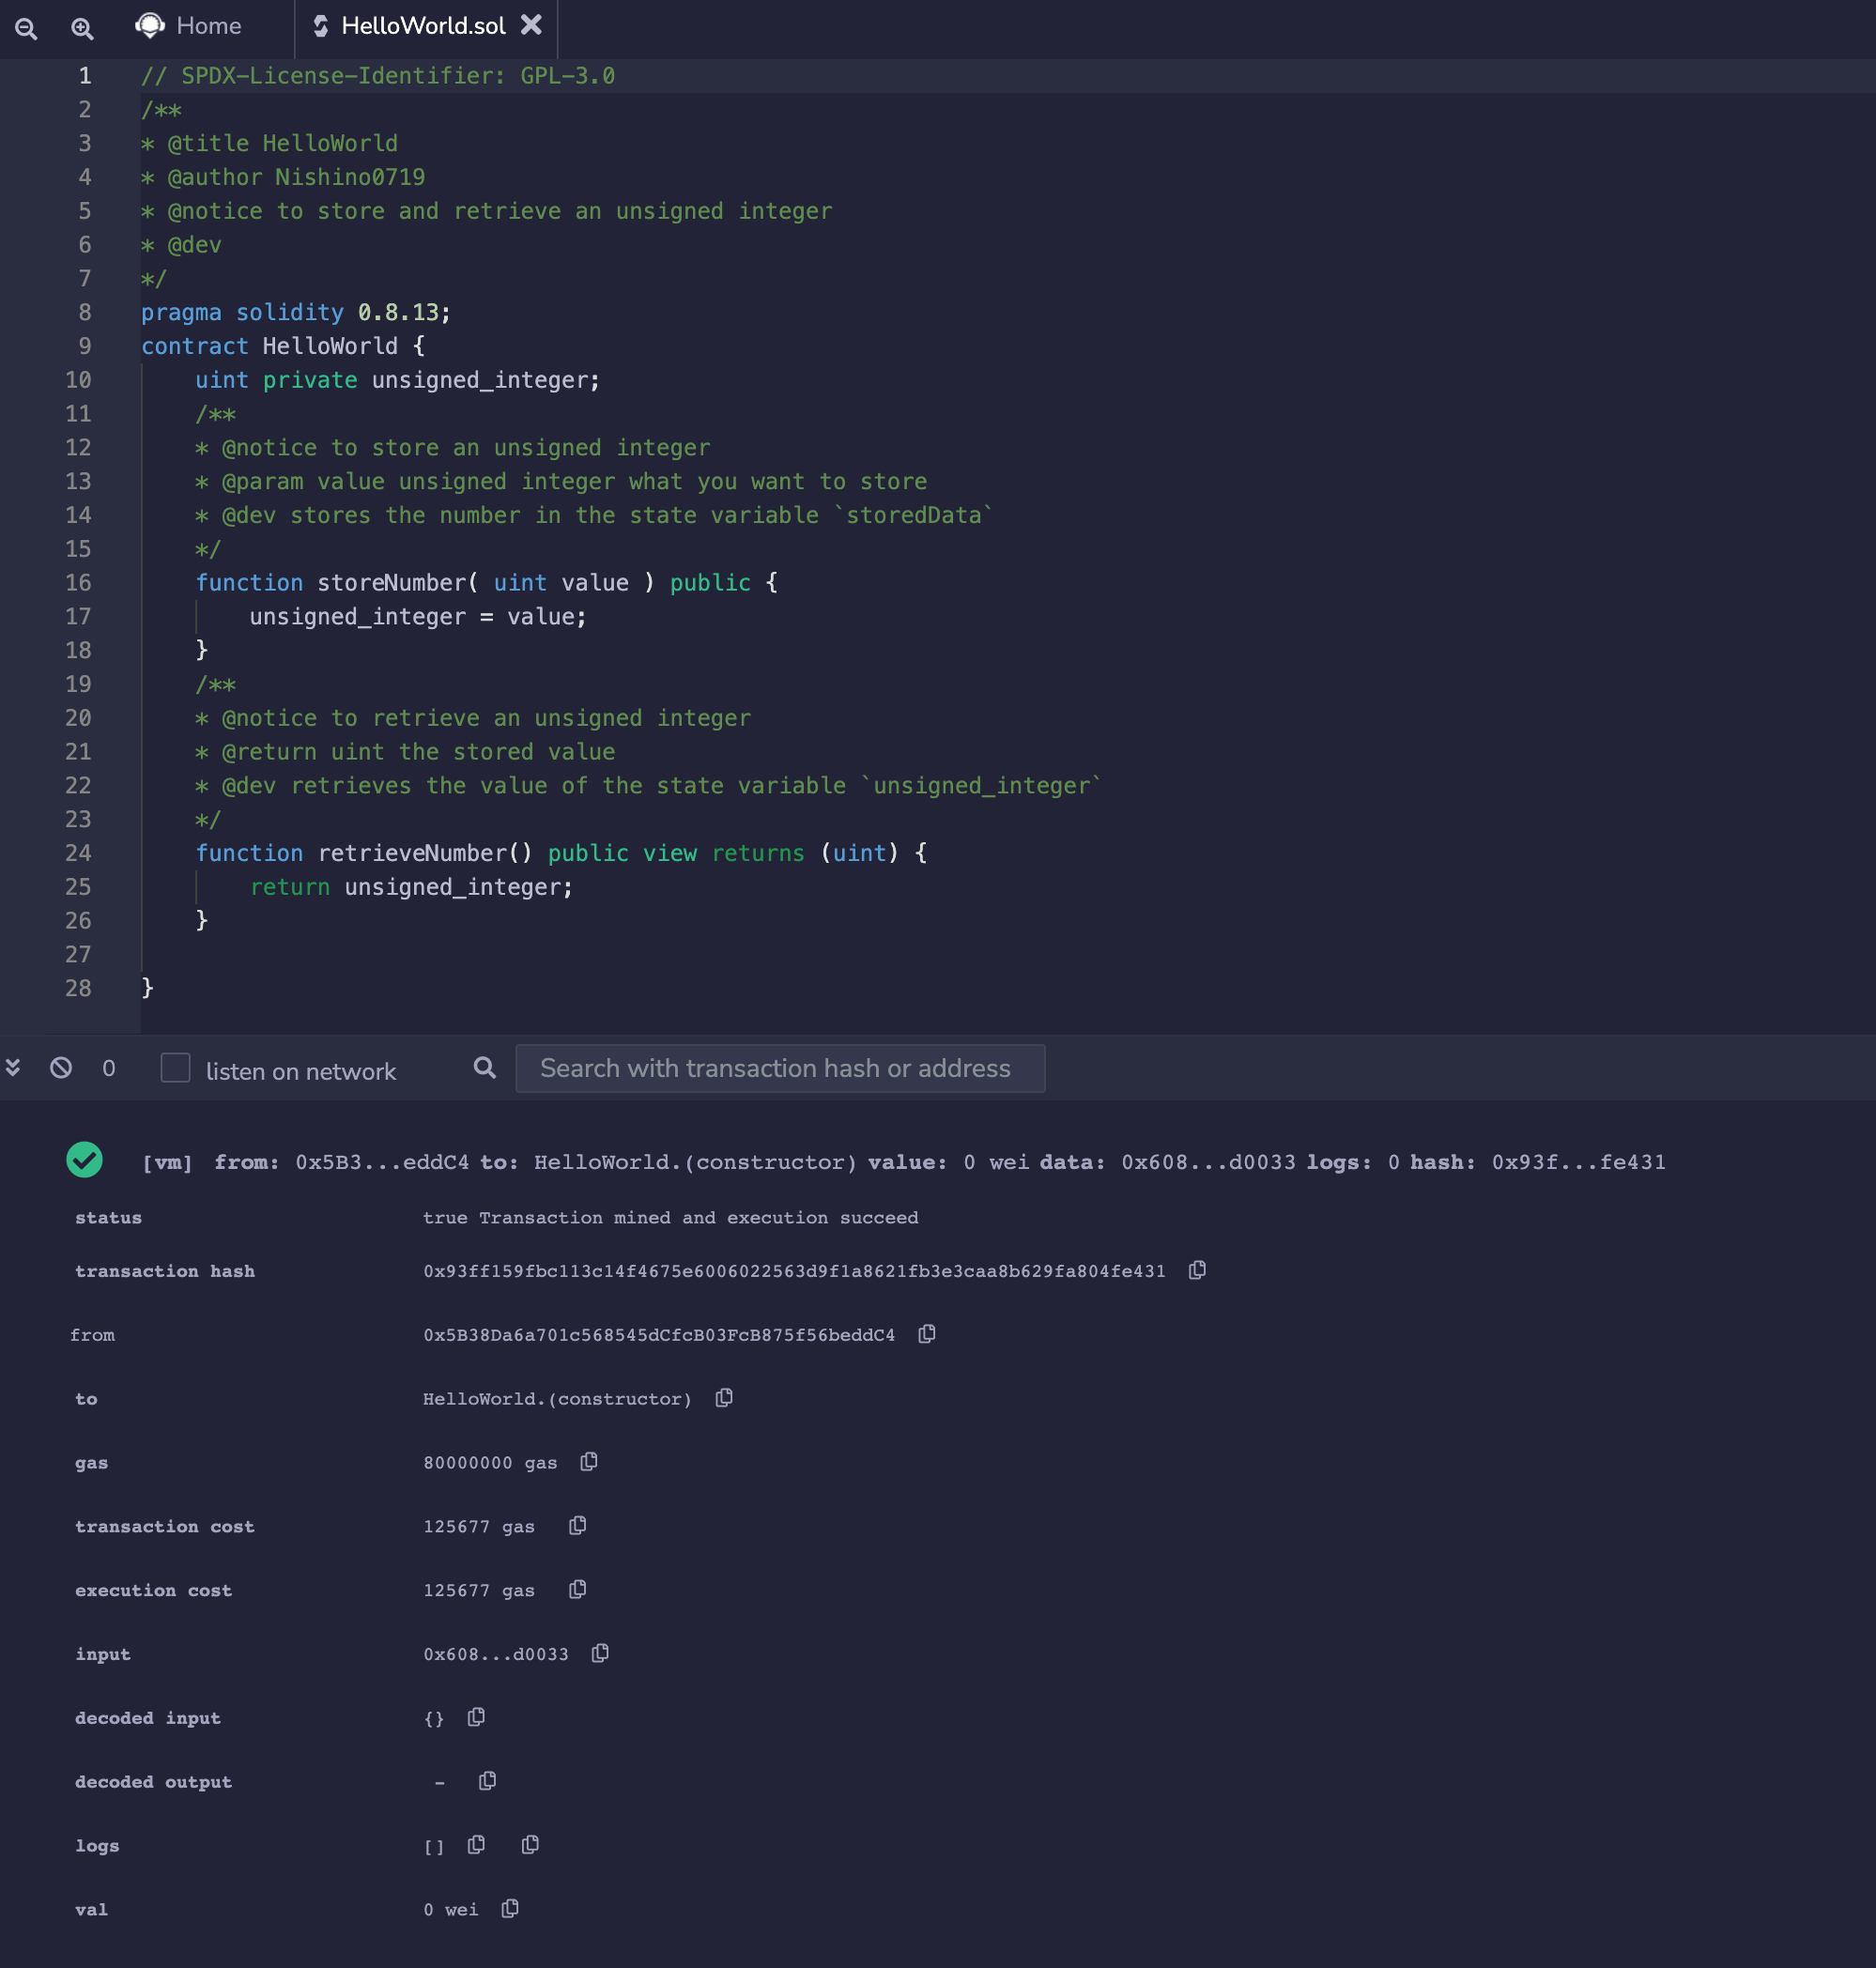
\includegraphics[width=\linewidth]{HelloWorld.png}
    \end{figure}
    \newpage
    \item \textbf{\large{Ballot: Suppose we want to limit the voting period of each Ballot contract to 5 minutes.}}\mbox{}\\
    Ballot.sol
    \newline
    Code: \href{https://github.com/Nishino0719/Zero-Knowledge-University/blob/main/BackgroundAssignment/B/Ballot.sol}{Code url}\mbox{}\\
    Commit: \href{https://github.com/Nishino0719/Zero-Knowledge-University/pull/2/commits/33740f496a53ee4d4b72f3ebaa7f93af42f2d31e}{Commit code url}\mbox{}\\
    Pull Request:\href{https://github.com/Nishino0719/Zero-Knowledge-University/pull/2/files}{https://github.com/Nishino0719/Zero-Knowledge-University/pull/2/files}
    \begin{figure}[h]
        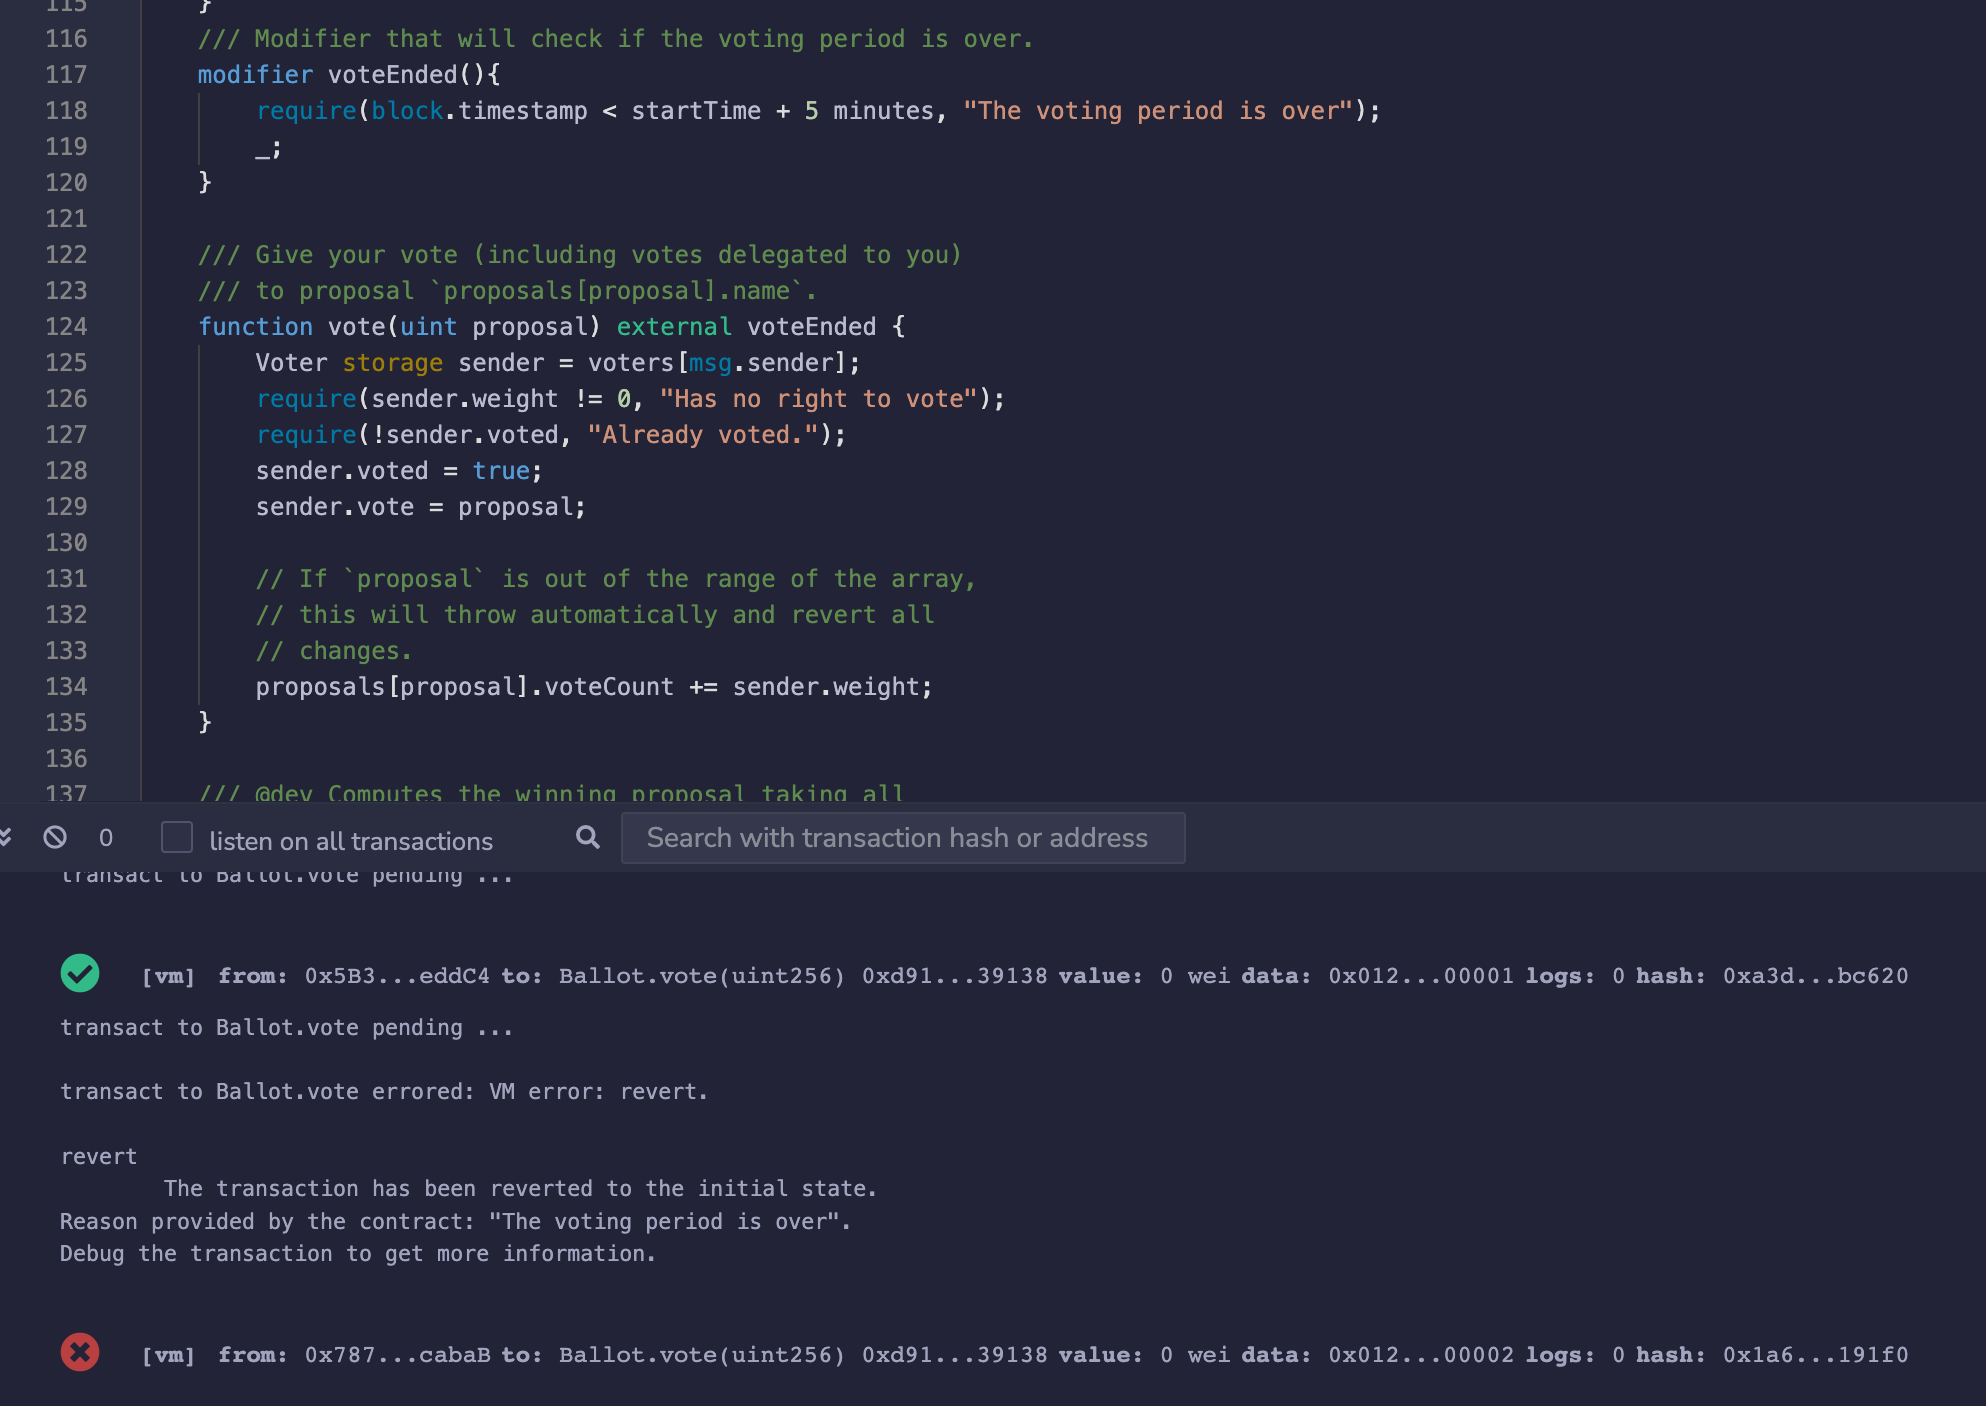
\includegraphics[width=\linewidth]{Ballot.png}
    \end{figure}
    
  \end{enumerate}


\end{document}